% Ensure included PDFs (banners) with newer versions embed without warnings
\pdfminorversion=7
\documentclass[aspectratio=169]{beamer}

\makeatletter
% Make LaTeX find theme .sty files in Template
\def\input@path{{../Template/}}
\makeatother
\usepackage{graphicx}
% Make graphics (including banner PDFs) resolvable without TEXINPUTS
\graphicspath{{../Template/}{../Template/banners/}{../../Common_Images/}}

%================================================================%
% Theme and Package Setup
%================================================================%
\usetheme{ucl}
\setbeamercolor{banner}{bg=darkpurple}

% Navigation and Footer
\setbeamertemplate{navigation symbols}{\vspace{-2ex}}
\setbeamertemplate{footline}[author title date]
\setbeamertemplate{slide counter}[framenumber/totalframenumber]

\usepackage[utf8]{inputenc}
\usepackage[british]{babel} % British spelling
\usepackage{amsmath, amssymb, amsthm}
\usepackage{graphicx}
\usepackage{tikz}
\usetikzlibrary{calc, positioning, arrows.meta, shapes.geometric, trees, backgrounds, shapes.misc, graphs, quotes, shadows, fit, patterns} 
\usepackage{pgfplots}
\pgfplotsset{compat=1.17}
\usefonttheme{professionalfonts}
\usepackage{eulervm}
\usepackage{listings}
\usepackage{algorithm}
\usepackage{algpseudocode}
\usepackage{xcolor}
\usepackage{subcaption}

% Define custom colours
\makeatletter
\@ifundefined{color@stone}{%
    \definecolor{stone}{gray}{0.95}%
}{}
\makeatother
\definecolor{darkgreen}{rgb}{0.0, 0.5, 0.0}
\definecolor{uclblue}{cmyk}{1,0.24,0,0.64}
\definecolor{uclred}{cmyk}{0,1,0.62,0}
\definecolor{uclpurple}{cmyk}{0.32,0.42,0,0.55}

\setbeamercovered{transparent}

% Define theoremblock
\makeatletter
\newenvironment<>{theoremblock}[1]{%
    \begin{block}#2{#1}%
}{\end{block}}
\makeatother

% Section divider slides
\AtBeginSection[]{
  \begin{frame}
    \frametitle{\textbf{\Large\insertsectionhead}}
    \begin{center}
        \huge\textbf{\insertsectionhead}
    \end{center}
  \end{frame}
}

% Maths Macros
\newcommand{\U}{\mathcal{U}}
\newcommand{\V}{\mathcal{V}}
\newcommand{\Z}{\mathcal{Z}}
\newcommand{\R}{\mathbb{R}}
\newcommand{\E}{\mathbb{E}}
\newcommand{\ip}[2]{\langle #1, #2 \rangle}
\newcommand{\norm}[1]{\| #1 \|}
\DeclareMathOperator*{\argmin}{argmin}
\DeclareMathOperator{\prox}{prox}
\DeclareMathOperator{\dom}{dom}
\DeclareMathOperator{\supremum}{sup}
\DeclareMathOperator{\sign}{sign}

\title{Deep Equilibrium Methods (DEQs)}
\subtitle{Part 1: Foundations, Universality, and the Forward Pass}
\author[Martin Benning (University College London)]{Martin Benning}
\date[COMP0263]{COMP0263 -- Solving Inverse Problems with Data-Driven Models \\[1cm] 10th March 2026}
\institute[]{University College London}

\begin{document}

% --- Title Frame ---
\begin{frame}
  \titlepage
\end{frame}

% --- Outline ---
\begin{frame}{Lecture Overview}
    \tableofcontents
\end{frame}

\section{The Memory Bottleneck \& Explicit Networks}

\begin{frame}{The Deep Learning Stack (Recap)}
    Most modern feedforward deep networks and unrolled architectures rely on \textbf{explicit layer stacking}.
    
    \begin{columns}
        \begin{column}{0.5\textwidth}
            \begin{itemize}
                \item \textbf{Forward pass:} Sequence of $L$ transformations.
                \item $L$ defines the depth or the algorithmic iteration budget.
                \item \textbf{Backward pass:} Relies on exact chain-rule backpropagation through all $L$ layers.
            \end{itemize}
        \end{column}
        \begin{column}{0.5\textwidth}
            % 
            \begin{figure}
                \centering
                \begin{tikzpicture}[scale=0.8, transform shape]
                    \node[draw, fill=uclblue!20, minimum width=3cm, minimum height=0.6cm] (l1) at (0,0) {Layer 1 ($f_{\theta_1}$)};
                    \node[draw, fill=uclblue!20, minimum width=3cm, minimum height=0.6cm] (l2) at (0,1.2) {Layer 2 ($f_{\theta_2}$)};
                    \node (dots) at (0,2.2) {$\vdots$};
                    \node[draw, fill=uclblue!20, minimum width=3cm, minimum height=0.6cm] (lL) at (0,3.2) {Layer $L$ ($f_{\theta_L}$)};
                    
                    \draw[->, thick] (0,-0.8) node[below]{Input $x$} -- (l1);
                    \draw[->, thick] (l1) -- (l2);
                    \draw[->, thick] (l2) -- (dots);
                    \draw[->, thick] (dots) -- (lL);
                    \draw[->, thick] (lL) -- (0,4.2) node[above]{Output};
                    
                    \draw[->, thick, uclred, dashed] (1.8, 3.2) to[bend left=30] node[right]{Backprop} (1.8, 1.2);
                \end{tikzpicture}
            \end{figure}
        \end{column}
    \end{columns}
\end{frame}

\begin{frame}{The $\mathcal{O}(L)$ Memory Bottleneck}
    To optimise explicit networks, backpropagation necessitates storing the intermediate activation values of \textbf{every single layer}.
    
    \vspace{1em}
    \begin{block}{The Hardware Limit}
        This creates an $\mathcal{O}(L)$ memory bottleneck that strictly limits:
        \begin{itemize}
            \item The capacity of the model.
            \item The resolution of images we can process.
            \item The absolute depth of the architectures we can train on modern GPUs.
        \end{itemize}
    \end{block}
\end{frame}

\begin{frame}{The Truncation Error Problem}
    Finite unrolling ties accuracy and depth directly to a pre-determined iteration budget $L$.
    
    \begin{columns}
        \begin{column}{0.55\textwidth}
            \uncover<2->{
                If an unrolled model requires \textbf{more} iterations to converge at inference time than it was trained for...
            }
            \vspace{1em}
            
            \uncover<3->{
                ...it suffers from severe \textbf{truncation errors} and \textbf{mathematical instability}.
            }
        \end{column}
        \begin{column}{0.45\textwidth}
            % 
            \uncover<3->{
                \begin{figure}
                    \centering
                    \begin{tikzpicture}
                        \begin{axis}[
                            width=0.9\textwidth, height=4.5cm,
                            xlabel={Inference Depth}, ylabel={Error},
                            ticks=none, axis lines=left,
                            xmin=0, xmax=10, ymin=0, ymax=10
                        ]
                        \addplot[domain=0:5, thick, darkgreen] {5*exp(-x) + 1};
                        \addplot[domain=5:9, thick, uclred] {1 + (x-5)^2};
                        \draw[dashed] (5,0) -- (5,10) node[pos=0.5, right] {Train Depth $L$};
                        \end{axis}
                    \end{tikzpicture}
                \end{figure}
            }
        \end{column}
    \end{columns}
\end{frame}

\section{Implicit Models \& The Equilibrium Equation}

\begin{frame}{The Paradigm Shift: Implicit Models}
    To overcome these memory and depth limitations, we undergo a profound shift in perspective.
    
    \vspace{1em}
    \begin{center}
        \Large \textbf{From} explicit algebraic layers \\
        \vspace{0.5em}
        \Large \textbf{To} continuous dynamics and implicit models \cite{bai2019deep}.
    \end{center}
    \vspace{1em}
    
    Instead of layers being side-effects of finite algorithms, \textbf{equilibrium conditions} become the central computational object.
\end{frame}

\begin{frame}{Historical Context: Recurrent Backpropagation}
    The foundational idea is not entirely new.
    
    \vspace{1em}
    It traces its roots back to the late 1980s with \textbf{recurrent backpropagation} \cite{almeida1987learning, pineda1987generalization}.
    
    \begin{itemize}
        \item Early works recognised network states could be driven to an equilibrium.
        \item \textbf{The limitation:} They were restricted to small-scale, fixed-input settings.
        \item They lacked the architectural complexity of modern deep learning.
    \end{itemize}
\end{frame}

\begin{frame}{Modern Deep Equilibrium Models (DEQs)}
    The modern DEQ framework \cite{bai2019deep} expresses the entire deep architecture as a \textbf{single, infinitely deep, weight-tied equilibrium computation}.
    
    \vspace{1em}
    Crucially, DEQs do not rely on slow, naive fixed-point iteration. 
    \vspace{1em}
    
    They utilise highly efficient \textbf{black-box root-finding algorithms} (like Broyden's method \cite{broyden1965class}) to solve for the fixed point directly \cite{kolter2020deepimplicit}.
\end{frame}

\begin{frame}{Visualising the Memory Footprint}
    \begin{figure}[htpb]
        \centering
        \begin{minipage}{0.32\textwidth}
            \centering
            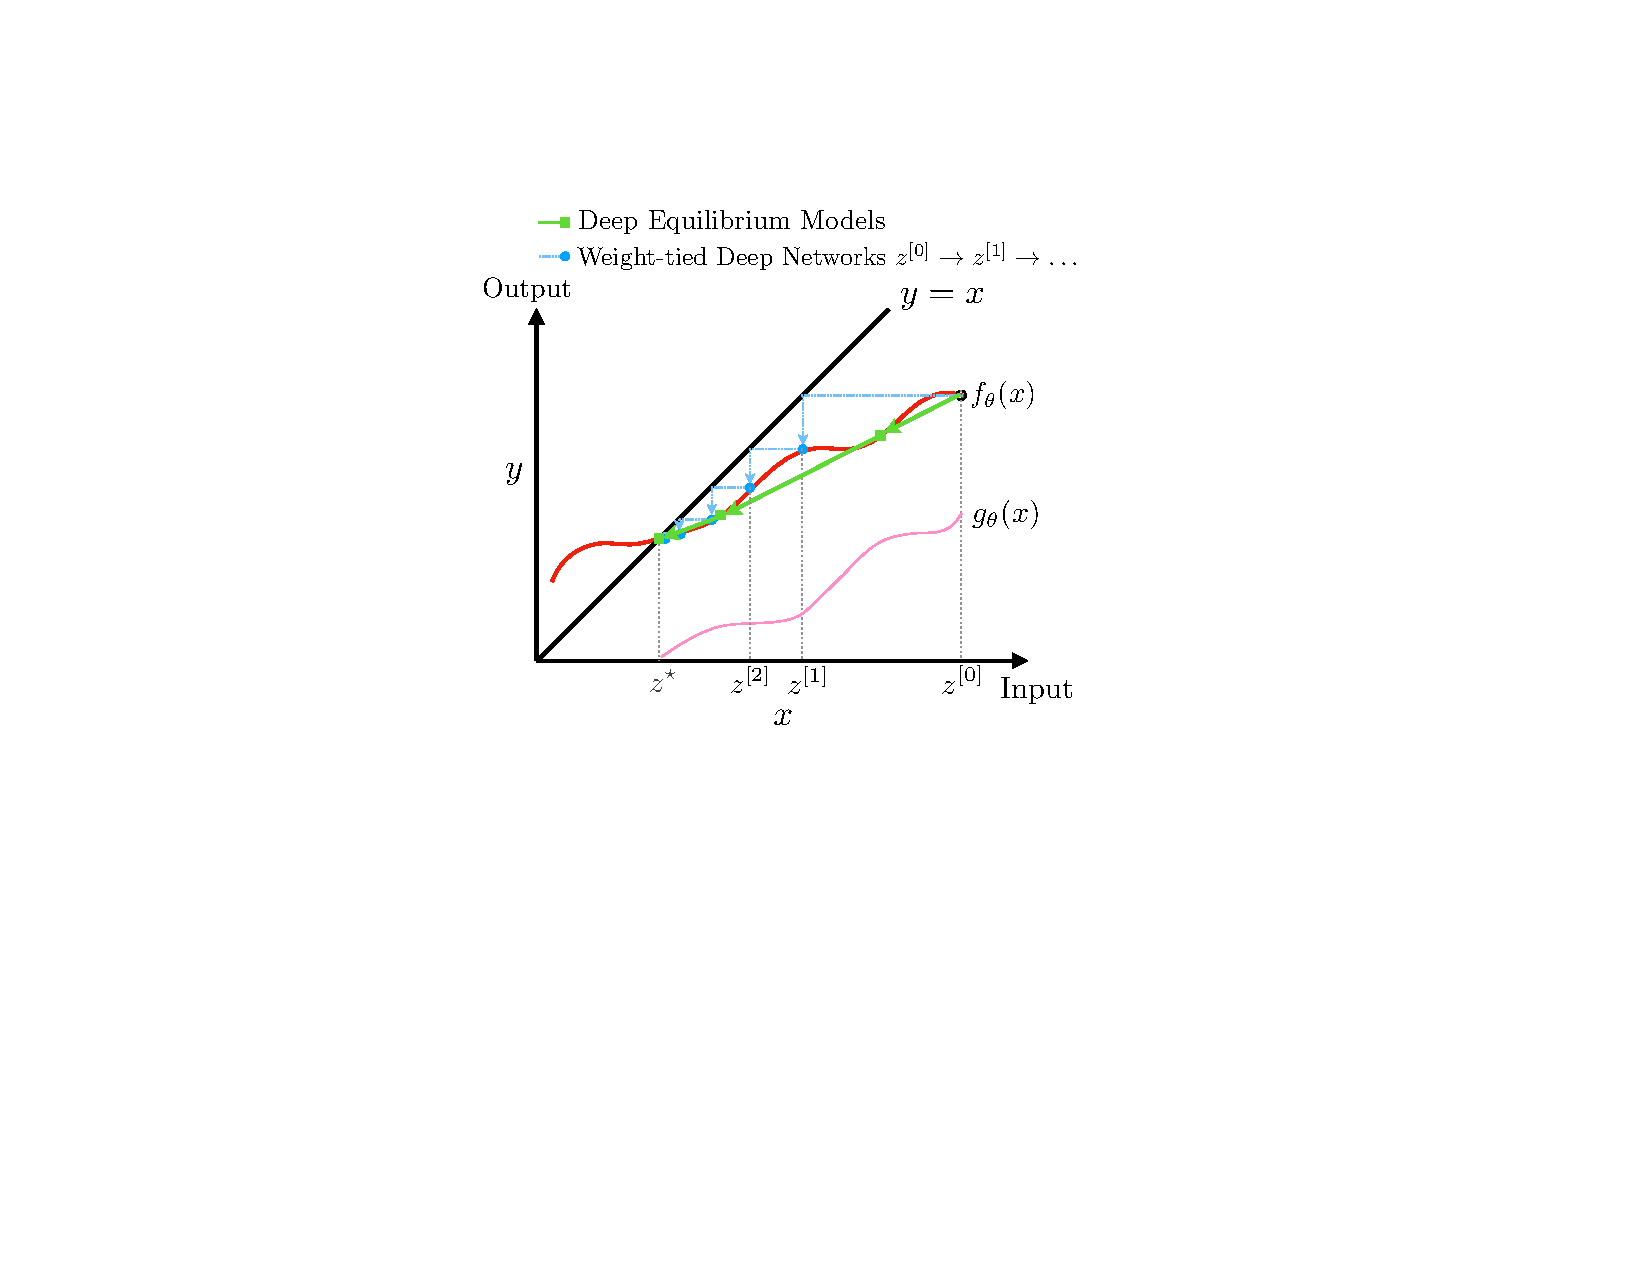
\includegraphics[width=\textwidth]{../Common_Images/deq/fp_onefig.pdf}
            \caption*{Solving for an equilibrium point in 2D.}
        \end{minipage}
        \hfill
        \begin{minipage}{0.6\textwidth}
            \centering
            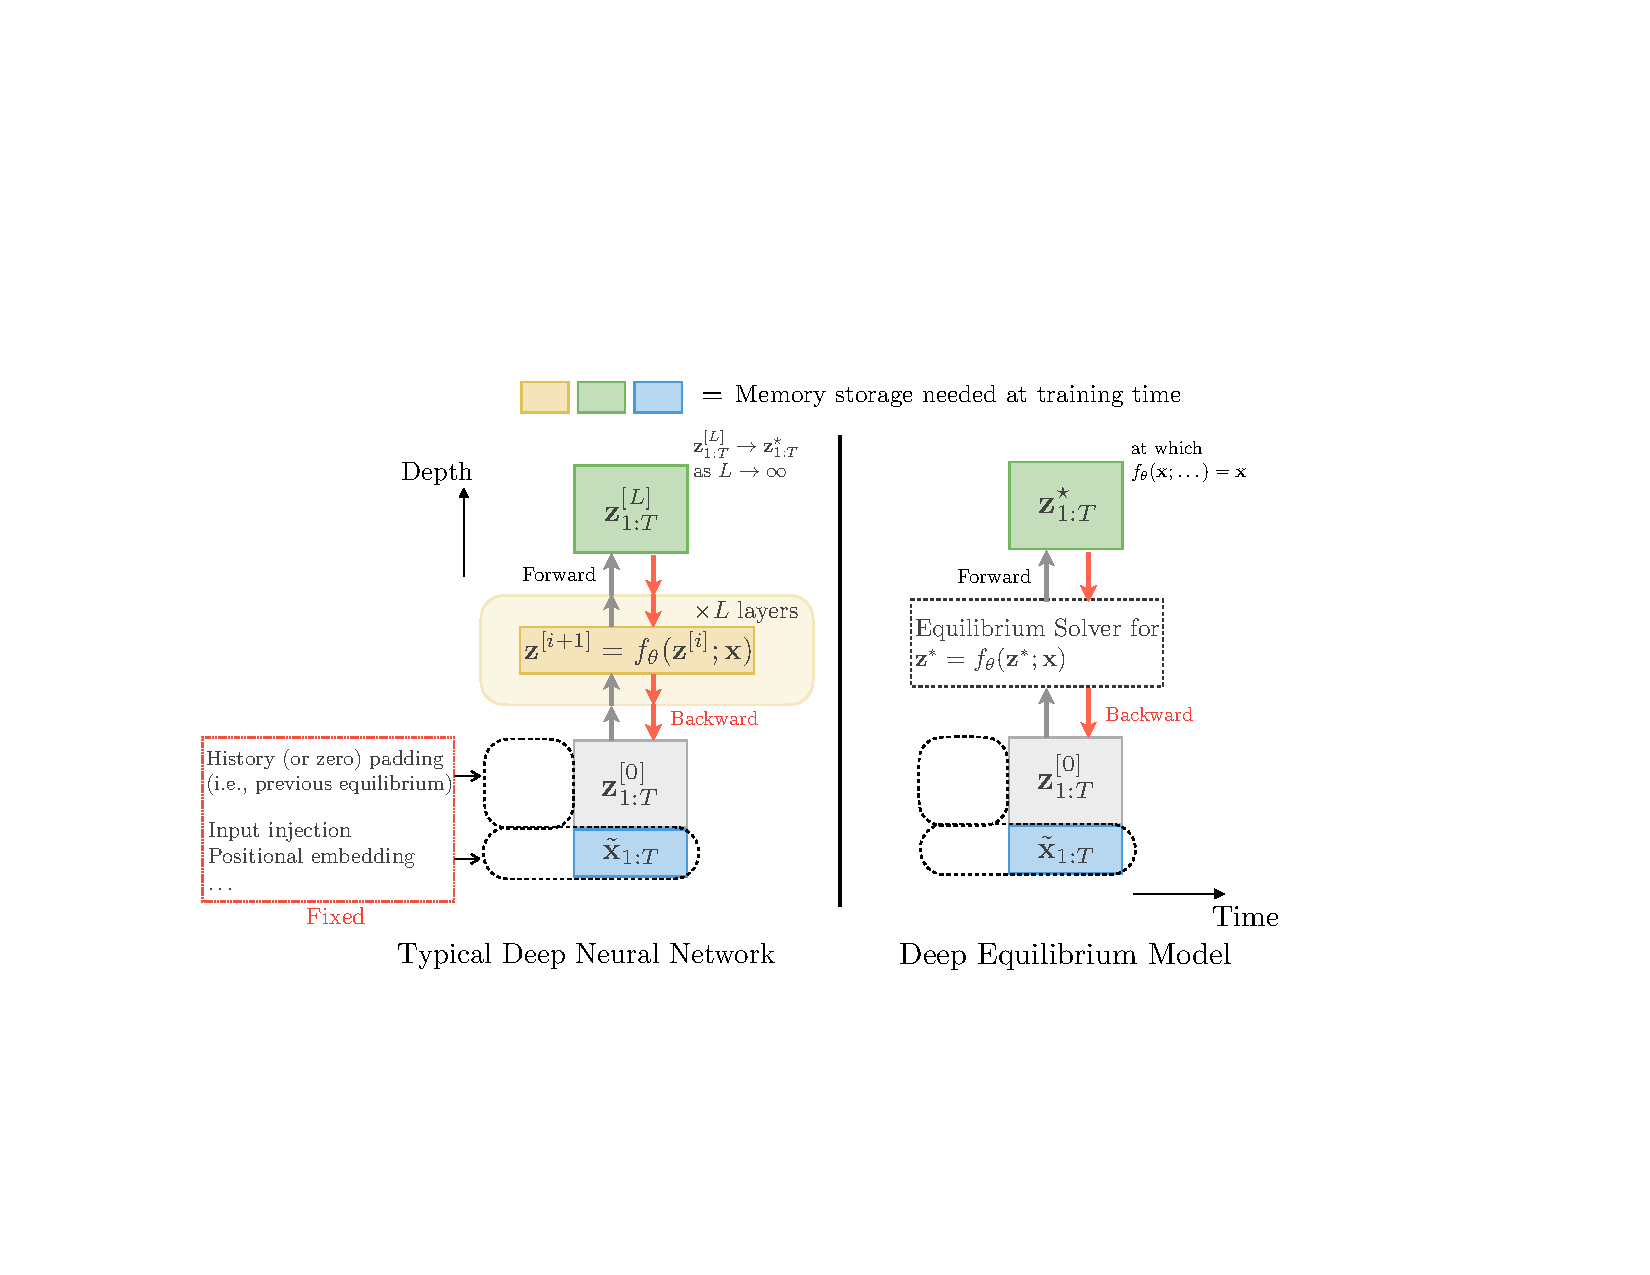
\includegraphics[width=\textwidth]{../Common_Images/deq/equm_vs_dnn.pdf}
            \caption*{DEQ vs conventional deep network memory.}
        \end{minipage}\vspace{-0.35cm}
        \caption{Explicit layers incur memory growth with depth. DEQs compute an equilibrium state with constant memory usage. From \cite{bai2019deep}.}
        \label{fig:deq_memory_footprint}
    \end{figure}
\end{frame}

\begin{frame}{The Equilibrium Equation}
    In an explicit network, layer transitions are written as
    $$ {\color{darkgreen}z}_{i+1} = f_{\color{uclblue}\theta_i}({\color{darkgreen}z}_i, {\color{uclred}x}) $$
    where ${\color{uclred}x}$ is the input, ${\color{darkgreen}z}_i$ the hidden state, and ${\color{uclblue}\theta_i}$ the parameters.
    
    \pause
    \vspace{1em}
    If weights are tied across depth (${\color{uclblue}\theta_i} = {\color{uclblue}\theta}$), an equilibrium state ${\color{darkgreen}z^\star}$ satisfies the fixed-point condition, which gives
    
    \begin{theoremblock}{The Fixed-Point Condition}
    $$ {\color{darkgreen}z^\star} = f_{\color{uclblue}\theta}({\color{darkgreen}z^\star}, {\color{uclred}x}) $$
    \end{theoremblock}
\end{frame}

\begin{frame}{From Fixed-Point to Root-Finding}
    While we can apply fixed-point iteration (Picard iteration) ${\color{darkgreen}z}_{i+1} = f_{\color{uclblue}\theta}({\color{darkgreen}z}_i, {\color{uclred}x})$, this is often too slow.
    
    \vspace{1em}
    DEQs typically recast the fixed-point condition as a \textbf{root-finding problem}. Defining the residual yields
    
    $$ g_{\color{uclblue}\theta}({\color{darkgreen}z^\star}, {\color{uclred}x}) := f_{\color{uclblue}\theta}({\color{darkgreen}z^\star}, {\color{uclred}x}) - {\color{darkgreen}z^\star} = 0 . $$
    
    \vspace{1em}
    This is then solved with accelerated black-box methods.
\end{frame}

\section{Representational Power (Universality)}

\begin{frame}{Representational Power: A Concern}
    \textbf{Question:} Does replacing explicit depth with a single implicit equilibrium condition reduce expressivity?
    
    \pause
    \vspace{1em}
    \textbf{Answer:} No. The DEQ perspective separates \emph{how} a representation is computed from \emph{what} representation is admissible at equilibrium.
    \vspace{1em}
    
    This separation allows a single implicit layer to encode transformations that would otherwise require many explicit layers.
\end{frame}

\begin{frame}{Universality of a Single DEQ Layer}
    Explicit depth can be absorbed into state dimension without exponential parameter growth.
    
    \vspace{1em}
    \begin{theoremblock}{Representational Corollary \cite{bai2019deep}}
        Consider a finite feedforward network of arbitrary depth acting on input $x$. There exists a DEQ map $f_\theta(\cdot; x)$ on an \textbf{augmented hidden state} such that the equilibrium state $z^\star$ encodes the same input-output mapping. The parameter count increases at most polynomially (often linearly), avoiding exponential blowup.
    \end{theoremblock}
\end{frame}

\begin{frame}{Stacking DEQ Layers: Setup}
    Suppose we define two implicit layers in sequence, producing
    $$ z^\star = f_{\theta_1}(z^\star; x) $$
    $$ y^\star = h_{\theta_2}(y^\star; z^\star) $$
    
    \vspace{1em}
    Can we increase expressivity by stacking multiple DEQ blocks like explicit layers?
\end{frame}

\begin{frame}{Equivalence of Stacked DEQs}
    We define a joint state $s = (z,y)$ and a joint map via
    $$ \Gamma_\Theta(s; x) := \big(f_{\theta_1}(z; x),\, h_{\theta_2}(y; z)\big), \qquad \Theta := (\theta_1,\theta_2) $$
    
    \pause
    The stacked system is equivalent to a single equilibrium condition, yielding
    $$ s^\star = \Gamma_\Theta(s^\star; x) $$
    
    \vspace{0.5em}
    \begin{theoremblock}{No Additional Expressive Power \cite{bai2019deep}}
        Any finite stack of DEQ blocks can be rewritten as one DEQ block on a concatenated hidden state. Stacked DEQs provide \textbf{no additional representational power} over a single DEQ layer of adequate width.
    \end{theoremblock}
\end{frame}

\begin{frame}{Shift in Architectural Design}
    Because macroscopic stacking yields no theoretical gain, our design focus shifts.
    
    \vspace{1em}
    \begin{itemize}
        \item \textbf{Old Paradigm:} How many layers do I stack?
        \item \textbf{DEQ Paradigm:} How do I design a highly expressive, stable transformation cell $f_\theta$?
    \end{itemize}
    \vspace{1em}
    
    Emphasis moves towards regularisation, stability, input injection, and injecting inductive biases appropriate for the task domain.
\end{frame}

\section{The Forward Pass \& Broyden's Method}

\begin{frame}{The Forward Pass: Solving $g_\theta = 0$}
    Because the output of a DEQ is simply the equilibrium point, the forward pass can utilise \textbf{any} black-box root-finding algorithm to solve
    
    $$ g_\theta(z^\star; x) = 0 $$
    
    \vspace{1em}
    \begin{itemize}
        \item The model output becomes \textbf{agnostic to the specific solver trajectory}.
        \item Well-posedness requires the existence of an equilibrium, and ideally uniqueness and local stability.
    \end{itemize}
\end{frame}

\begin{frame}{Picard Iteration \& Its Limits}
    Standard fixed-point iteration (Picard iteration) updates via
    $$ z_{k+1} = f_\theta(z_k; x) $$
    
    \vspace{1em}
    Local convergence is guaranteed if the spectral radius of the Jacobian $\rho(J_{f_\theta}) < 1$ (Banach's fixed-point theorem).
    
    \vspace{1em}
    \begin{alertblock}{The Problem}
        While this provides theoretical guarantees for strict contractions, its \textbf{linear convergence rate} is often far too slow for practical deep learning applications.
    \end{alertblock}
\end{frame}

\begin{frame}{Newton's Method}
    A more efficient strategy shifts to root-finding for the residual function $g_\theta(z; x) = z - f_\theta(z; x) = 0$.
    
    \vspace{1em}
    Newton's method leverages first-order derivative information via the Jacobian matrix $J_{g_\theta} = \partial_z g_\theta$. This yields the update
    
    $$ z_{k+1} = z_k - J_{g_\theta}(z_k;x)^{-1} g_\theta(z_k;x) $$
\end{frame}

\begin{frame}{The Jacobian Bottleneck}
    % 
    \begin{columns}
        \begin{column}{0.4\textwidth}
            Explicitly forming and inverting the $d \times d$ Jacobian matrix $J_{g_\theta}$ is \textbf{computationally infeasible} at the scale of modern deep neural networks.
            
            \vspace{1em}
            Here, $d$ represents the hidden state dimension, which can easily be in the millions. We need a method to approximate this inverse without constructing it.
        \end{column}
        \begin{column}{0.6\textwidth}
            \begin{figure}
                \centering
                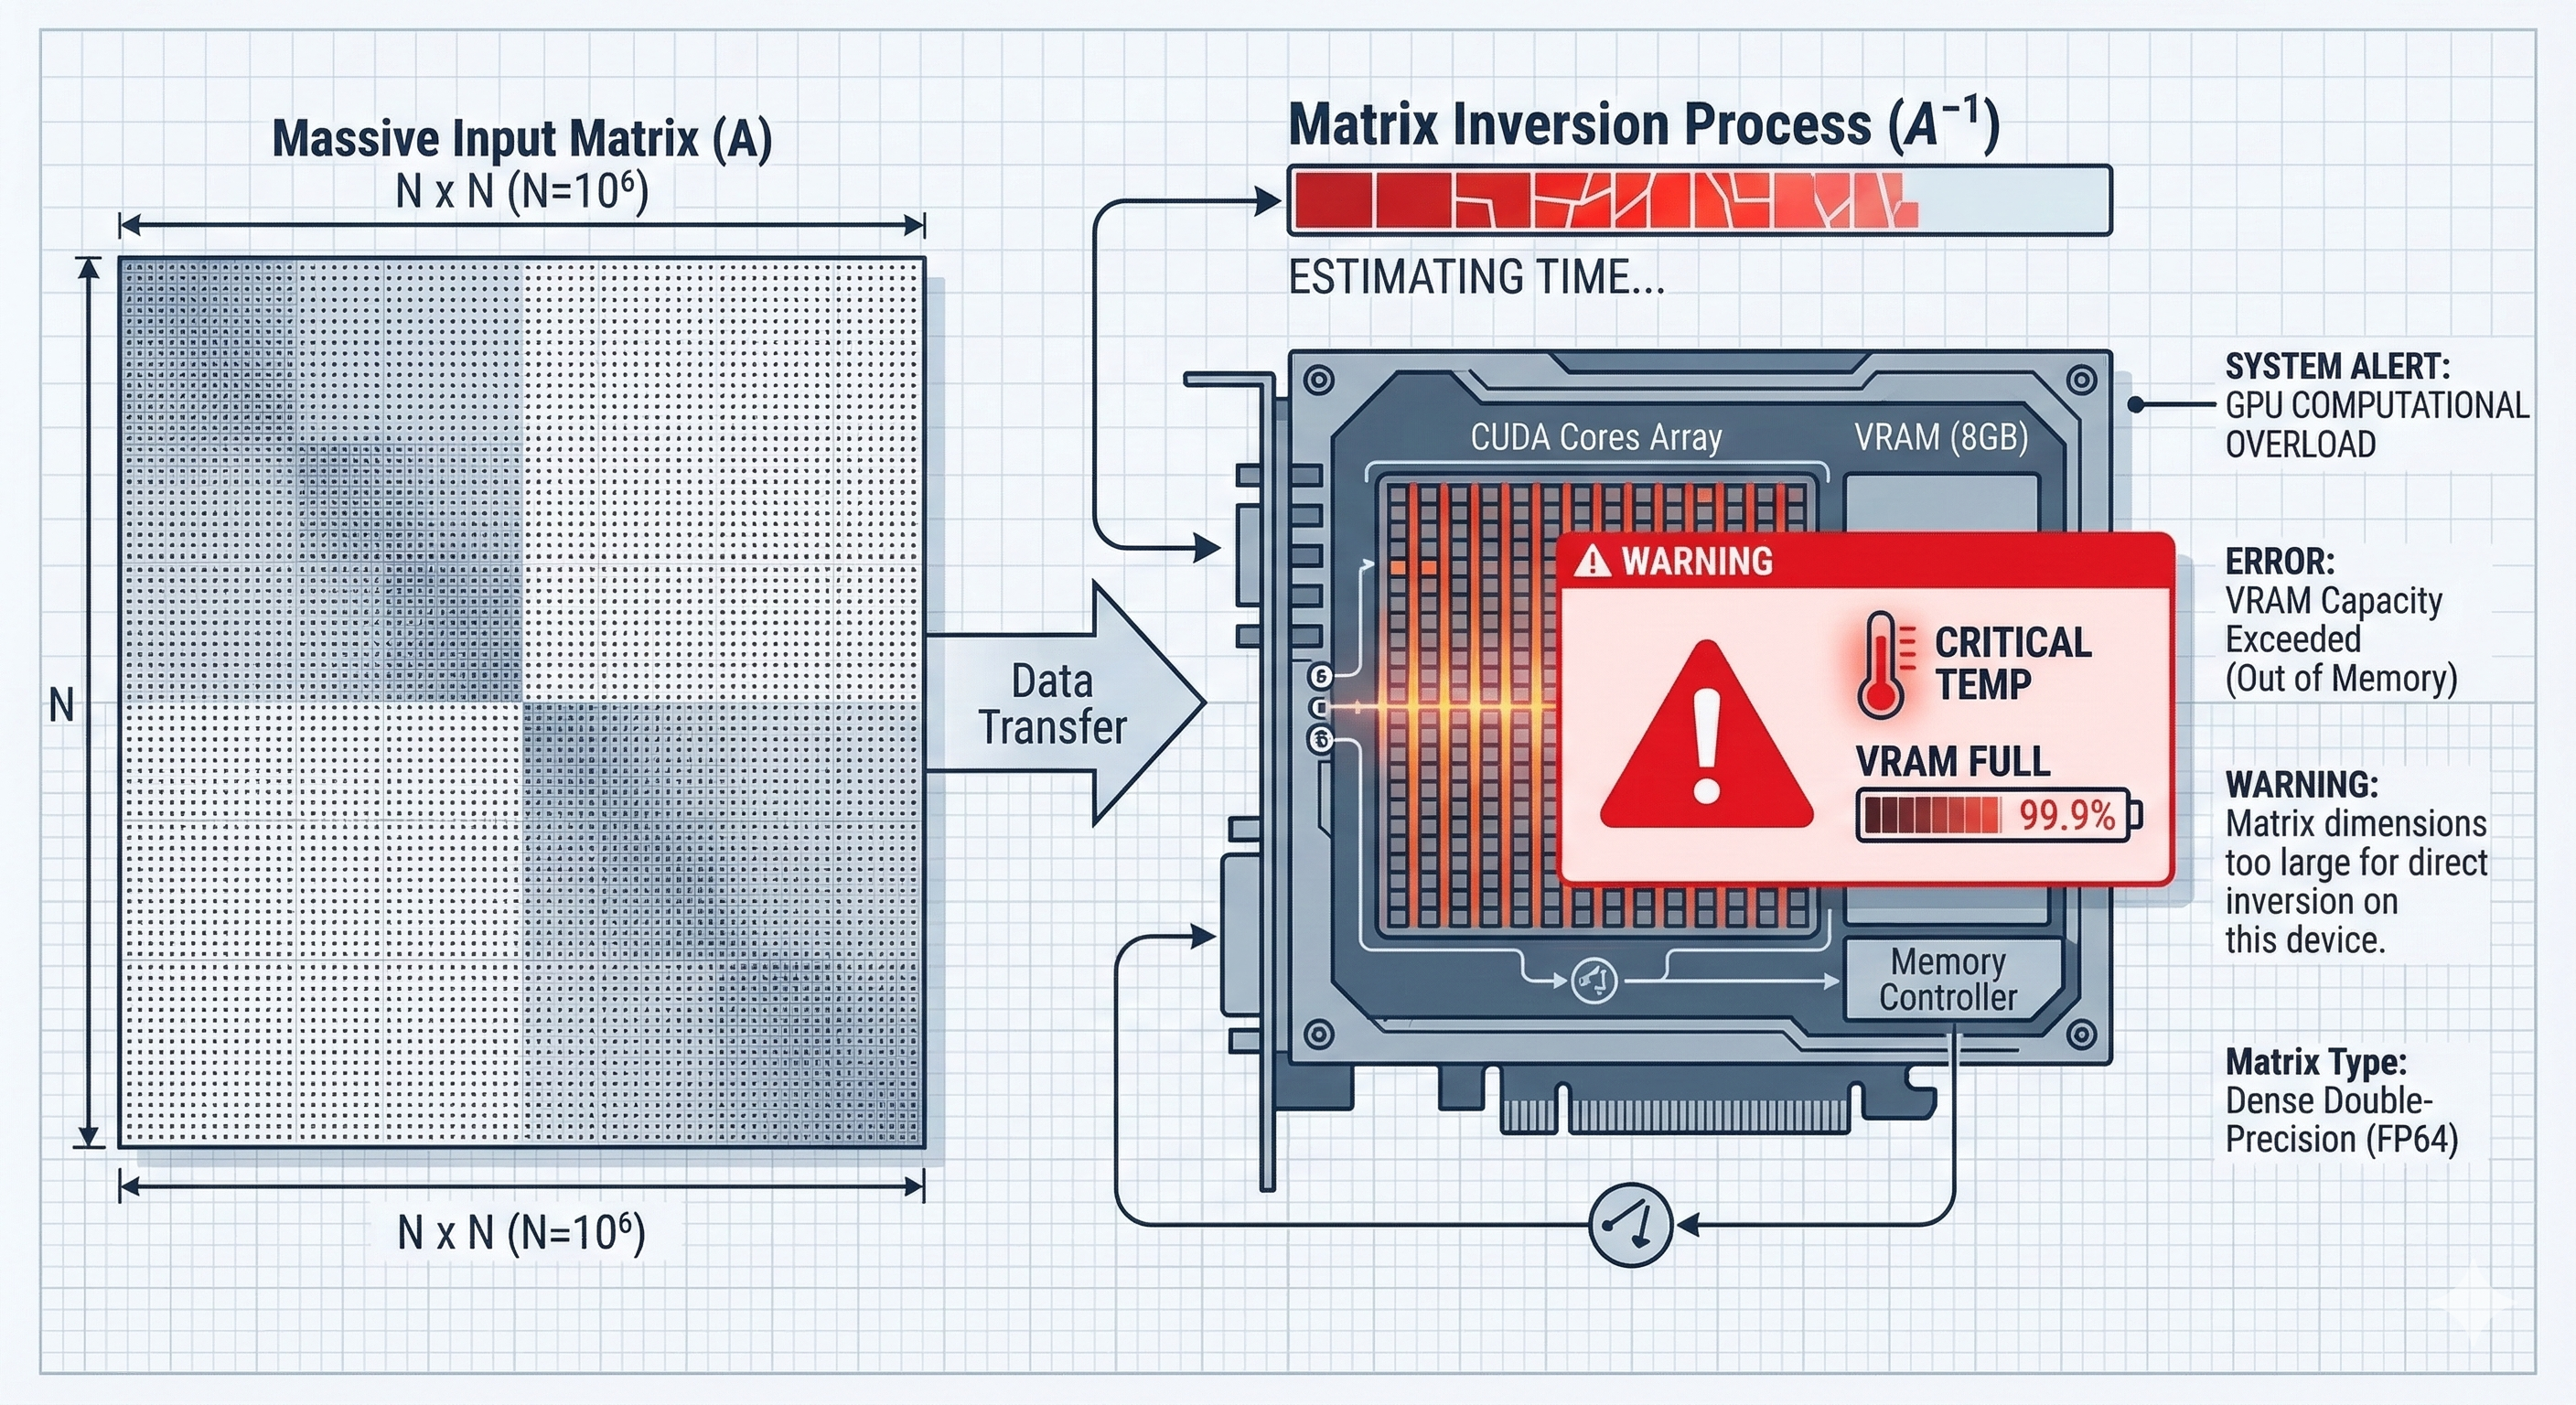
\includegraphics[width=\textwidth]{deq/largematrix.png}
                \caption*{Generated with Nano Banana Pro}
            \end{figure}
        \end{column}
    \end{columns}
\end{frame}

\begin{frame}{Broyden's Method: A Quasi-Newton Approach}
    Broyden's method \cite{broyden1965class} acts as a \emph{quasi-Newton} method, replacing the exact inverse Jacobian with an iterative approximation 
    
    $$H_k \approx J_{g_\theta}(z_k;x)^{-1} . $$
    
    \vspace{1em}
    This generalises the 1D secant method, where the derivative is approximated via finite differences:
    $$ f'(x_k) \approx \frac{f(x_k) - f(x_{k-1})}{x_k - x_{k-1}} . $$
\end{frame}

\begin{frame}{The Inverse Secant Condition}
    Define the step differences as:
    $$ \Delta z_k := z_k-z_{k-1} \qquad \text{and} \qquad \Delta g_k := g_k-g_{k-1} . $$
    
    \pause
    The equivalent condition on the approximated Jacobian $B_k \approx J_{g_\theta}$ is the secant equation $B_k \Delta z_k = \Delta g_k$.
    
    \pause
    \vspace{1em}
    Multiplying by the inverse approximation $H_k = B_k^{-1}$ produces the \textbf{inverse secant condition}
    $$ H_k \Delta g_k = \Delta z_k . $$
    
    \vspace{1em}
    \emph{Note:} This imposes only $d$ equations on a $d \times d$ matrix, leaving the system dramatically underdetermined!
\end{frame}

\begin{frame}{Formulating Broyden's Update}
    Broyden resolved this by proposing that $H_k$ should satisfy the secant equation while deviating \textbf{as little as possible} from the previous estimate $H_{k-1}$.
    
    \vspace{1em}
    This translates into a constrained minimisation problem:
    
    $$ \min_{H_k} \frac{1}{2}\|H_k - H_{k-1}\|_F^2 \quad \text{subject to} \quad H_k \Delta g_k = \Delta z_k . $$
\end{frame}

\begin{frame}{Deriving the Rank-One Update}
    We introduce a Lagrange multiplier vector $\lambda \in \R^d$ to form the Lagrangian. Setting the gradient with respect to $H_k$ to zero gives
    
    $$ H_k = H_{k-1} + \lambda \Delta g_k^{\top} . $$
    
    This explicitly reveals the update is inherently a \textbf{rank-one matrix}.
    
    \pause
    \vspace{1em}
    Substituting this back into the secant constraint and solving for $\lambda$ yields the recursive Broyden update
    
    \begin{theoremblock}{Broyden's Update}
    $$ H_k = H_{k-1} + \frac{(\Delta z_k-H_{k-1}\Delta g_k)\,\Delta g_k^{\top}}{\|\Delta g_k\|_2^2} $$
    \end{theoremblock}
\end{frame}

\begin{frame}{Practical Application of Broyden's}
    A crucial computational detail: computing the step $z_{k+1} = z_k - H_k g_k$ \textbf{does not} require instantiating the dense matrix $H_k$ in memory!
    
    \vspace{1em}
    \begin{itemize}
        \item $H_k$ is constructed entirely from successive rank-one updates starting from an initial guess (e.g., $H_0 = -I$).
        \item The matrix-vector product $H_k g_k$ can be evaluated efficiently using \textbf{only vector inner products}.
    \end{itemize}
\end{frame}

\begin{frame}{Limited-Memory Broyden (L-Broyden)}
    In DEQ implementations, this is pushed further by using \textbf{Limited-memory Broyden}.
    
    \vspace{1em}
    \begin{itemize}
        \item Stores only the most recent $m$ secant pairs $\{(\Delta z_i, \Delta g_i)\}_{i=k-m+1}^k$.
        \item Older pairs are discarded, bringing the memory footprint from $\mathcal{O}(d^2)$ strictly down to $\mathcal{O}(md)$ \cite{bai2019deep}.
        \item Unlike Picard iterations, Broyden only requires the residual's Jacobian to be non-singular (i.e., $1$ is not an eigenvalue).
    \end{itemize}
\end{frame}

\begin{frame}{Summary of Lecture 1}
    \begin{itemize}
        \item \textbf{The Bottleneck:} Explicit architectures suffer from an $\mathcal{O}(L)$ memory bottleneck and test-time truncation errors.
        \item \textbf{Implicit Paradigm:} DEQs replace finite explicit layers with a single, weight-tied equilibrium condition: $z^\star = f_\theta(z^\star, x)$.
        \item \textbf{Universality:} A single implicit layer is universally expressive; macroscopic stacking provides no theoretical gain.
        \item \textbf{Forward Pass:} Formulated as a root-finding problem ($g_\theta = 0$), solved efficiently with matrix-free algorithms like L-Broyden.
    \end{itemize}
    \vspace{1em}
    \textbf{Next Lecture:} We will explore the backward pass using implicit differentiation, ensuring $\mathcal{O}(1)$ memory training, and apply DEQs to sequence modelling!
\end{frame}

\begin{frame}[allowframebreaks]{References}
    \bibliographystyle{abbrv}
    \bibliography{../../Lecture_Notes/references}
\end{frame}

\end{document}